\documentclass[1p]{elsarticle_modified}
%\bibliographystyle{elsarticle-num}

%\usepackage[colorlinks]{hyperref}
%\usepackage{abbrmath_seonhwa} %\Abb, \Ascr, \Acal ,\Abf, \Afrak
\usepackage{amsfonts}
\usepackage{amssymb}
\usepackage{amsmath}
\usepackage{amsthm}
\usepackage{scalefnt}
\usepackage{amsbsy}
\usepackage{kotex}
\usepackage{caption}
\usepackage{subfig}
\usepackage{color}
\usepackage{graphicx}
\usepackage{xcolor} %% white, black, red, green, blue, cyan, magenta, yellow
\usepackage{float}
\usepackage{setspace}
\usepackage{hyperref}

\usepackage{tikz}
\usetikzlibrary{arrows}

\usepackage{multirow}
\usepackage{array} % fixed length table
\usepackage{hhline}

%%%%%%%%%%%%%%%%%%%%%
\makeatletter
\renewcommand*\env@matrix[1][\arraystretch]{%
	\edef\arraystretch{#1}%
	\hskip -\arraycolsep
	\let\@ifnextchar\new@ifnextchar
	\array{*\c@MaxMatrixCols c}}
\makeatother %https://tex.stackexchange.com/questions/14071/how-can-i-increase-the-line-spacing-in-a-matrix
%%%%%%%%%%%%%%%

\usepackage[normalem]{ulem}

\newcommand{\msout}[1]{\ifmmode\text{\sout{\ensuremath{#1}}}\else\sout{#1}\fi}
%SOURCE: \msout is \stkout macro in https://tex.stackexchange.com/questions/20609/strikeout-in-math-mode

\newcommand{\cancel}[1]{
	\ifmmode
	{\color{red}\msout{#1}}
	\else
	{\color{red}\sout{#1}}
	\fi
}

\newcommand{\add}[1]{
	{\color{blue}\uwave{#1}}
}

\newcommand{\replace}[2]{
	\ifmmode
	{\color{red}\msout{#1}}{\color{blue}\uwave{#2}}
	\else
	{\color{red}\sout{#1}}{\color{blue}\uwave{#2}}
	\fi
}

\newcommand{\Sol}{\mathcal{S}} %segment
\newcommand{\D}{D} %diagram
\newcommand{\A}{\mathcal{A}} %arc


%%%%%%%%%%%%%%%%%%%%%%%%%%%%%5 test

\def\sl{\operatorname{\textup{SL}}(2,\Cbb)}
\def\psl{\operatorname{\textup{PSL}}(2,\Cbb)}
\def\quan{\mkern 1mu \triangleright \mkern 1mu}

\theoremstyle{definition}
\newtheorem{thm}{Theorem}[section]
\newtheorem{prop}[thm]{Proposition}
\newtheorem{lem}[thm]{Lemma}
\newtheorem{ques}[thm]{Question}
\newtheorem{cor}[thm]{Corollary}
\newtheorem{defn}[thm]{Definition}
\newtheorem{exam}[thm]{Example}
\newtheorem{rmk}[thm]{Remark}
\newtheorem{alg}[thm]{Algorithm}

\newcommand{\I}{\sqrt{-1}}
\begin{document}

%\begin{frontmatter}
%
%\title{Boundary parabolic representations of knots up to 8 crossings}
%
%%% Group authors per affiliation:
%\author{Yunhi Cho} 
%\address{Department of Mathematics, University of Seoul, Seoul, Korea}
%\ead{yhcho@uos.ac.kr}
%
%
%\author{Seonhwa Kim} %\fnref{s_kim}}
%\address{Center for Geometry and Physics, Institute for Basic Science, Pohang, 37673, Korea}
%\ead{ryeona17@ibs.re.kr}
%
%\author{Hyuk Kim}
%\address{Department of Mathematical Sciences, Seoul National University, Seoul 08826, Korea}
%\ead{hyukkim@snu.ac.kr}
%
%\author{Seokbeom Yoon}
%\address{Department of Mathematical Sciences, Seoul National University, Seoul, 08826,  Korea}
%\ead{sbyoon15@snu.ac.kr}
%
%\begin{abstract}
%We find all boundary parabolic representation of knots up to 8 crossings.
%
%\end{abstract}
%\begin{keyword}
%    \MSC[2010] 57M25 
%\end{keyword}
%
%\end{frontmatter}

%\linenumbers
%\tableofcontents
%
\newcommand\colored[1]{\textcolor{white}{\rule[-0.35ex]{0.8em}{1.4ex}}\kern-0.8em\color{red} #1}%
%\newcommand\colored[1]{\textcolor{white}{ #1}\kern-2.17ex	\textcolor{white}{ #1}\kern-1.81ex	\textcolor{white}{ #1}\kern-2.15ex\color{red}#1	}

{\Large $\underline{12a_{1077}~(K12a_{1077})}$}

\setlength{\tabcolsep}{10pt}
\renewcommand{\arraystretch}{1.6}
\vspace{1cm}\begin{tabular}{m{100pt}>{\centering\arraybackslash}m{274pt}}
\multirow{5}{120pt}{
	\centering
	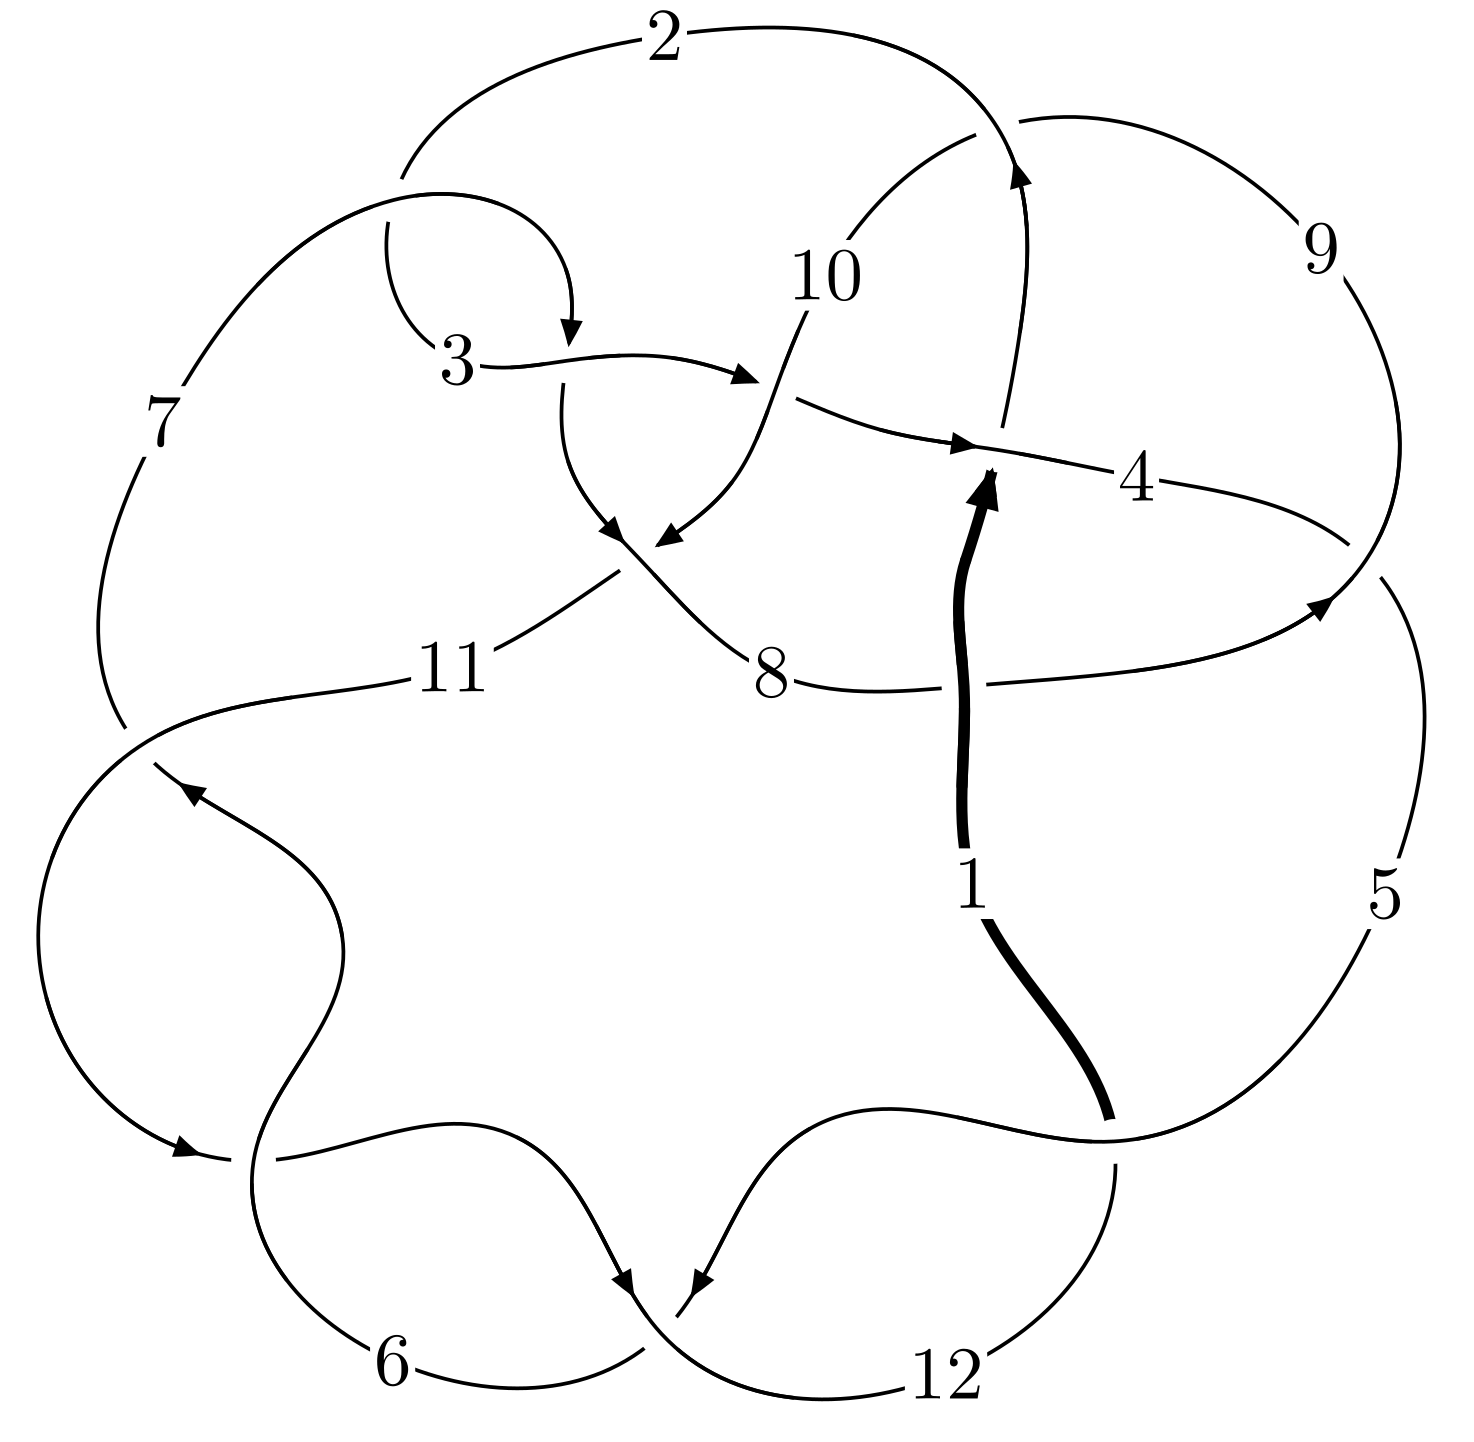
\includegraphics[width=112pt]{../../../GIT/diagram.site/Diagrams/png/1878_12a_1077.png}\\
\ \ \ A knot diagram\footnotemark}&
\allowdisplaybreaks
\textbf{Linearized knot diagam} \\
\cline{2-2}
 &
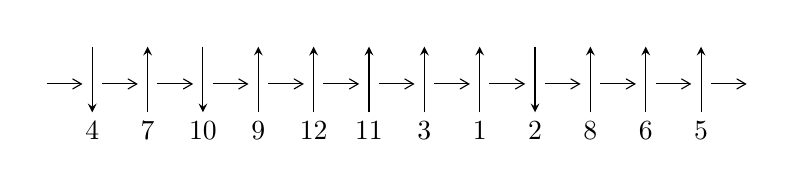
\begin{tikzpicture}[x=20pt, y=17pt]
	% nodes
	\node (C0) at (0, 0) {};
	\node (C1) at (1, 0) {};
	\node (C1U) at (1, +1) {};
	\node (C1D) at (1, -1) {4};

	\node (C2) at (2, 0) {};
	\node (C2U) at (2, +1) {};
	\node (C2D) at (2, -1) {7};

	\node (C3) at (3, 0) {};
	\node (C3U) at (3, +1) {};
	\node (C3D) at (3, -1) {10};

	\node (C4) at (4, 0) {};
	\node (C4U) at (4, +1) {};
	\node (C4D) at (4, -1) {9};

	\node (C5) at (5, 0) {};
	\node (C5U) at (5, +1) {};
	\node (C5D) at (5, -1) {12};

	\node (C6) at (6, 0) {};
	\node (C6U) at (6, +1) {};
	\node (C6D) at (6, -1) {11};

	\node (C7) at (7, 0) {};
	\node (C7U) at (7, +1) {};
	\node (C7D) at (7, -1) {3};

	\node (C8) at (8, 0) {};
	\node (C8U) at (8, +1) {};
	\node (C8D) at (8, -1) {1};

	\node (C9) at (9, 0) {};
	\node (C9U) at (9, +1) {};
	\node (C9D) at (9, -1) {2};

	\node (C10) at (10, 0) {};
	\node (C10U) at (10, +1) {};
	\node (C10D) at (10, -1) {8};

	\node (C11) at (11, 0) {};
	\node (C11U) at (11, +1) {};
	\node (C11D) at (11, -1) {6};

	\node (C12) at (12, 0) {};
	\node (C12U) at (12, +1) {};
	\node (C12D) at (12, -1) {5};
	\node (C13) at (13, 0) {};

	% arrows
	\draw[->,>={angle 60}]
	(C0) edge (C1) (C1) edge (C2) (C2) edge (C3) (C3) edge (C4) (C4) edge (C5) (C5) edge (C6) (C6) edge (C7) (C7) edge (C8) (C8) edge (C9) (C9) edge (C10) (C10) edge (C11) (C11) edge (C12) (C12) edge (C13) ;	\draw[->,>=stealth]
	(C1U) edge (C1D) (C2D) edge (C2U) (C3U) edge (C3D) (C4D) edge (C4U) (C5D) edge (C5U) (C6D) edge (C6U) (C7D) edge (C7U) (C8D) edge (C8U) (C9U) edge (C9D) (C10D) edge (C10U) (C11D) edge (C11U) (C12D) edge (C12U) ;
	\end{tikzpicture} \\
\hhline{~~} \\& 
\textbf{Solving Sequence} \\ \cline{2-2} 
 &
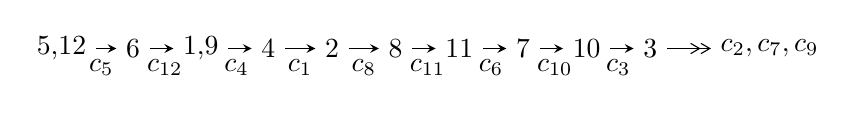
\begin{tikzpicture}[x=23pt, y=7pt]
	% node
	\node (A0) at (-1/8, 0) {5,12};
	\node (A1) at (1, 0) {6};
	\node (A2) at (33/16, 0) {1,9};
	\node (A3) at (25/8, 0) {4};
	\node (A4) at (33/8, 0) {2};
	\node (A5) at (41/8, 0) {8};
	\node (A6) at (49/8, 0) {11};
	\node (A7) at (57/8, 0) {7};
	\node (A8) at (65/8, 0) {10};
	\node (A9) at (73/8, 0) {3};
	\node (C1) at (1/2, -1) {$c_{5}$};
	\node (C2) at (3/2, -1) {$c_{12}$};
	\node (C3) at (21/8, -1) {$c_{4}$};
	\node (C4) at (29/8, -1) {$c_{1}$};
	\node (C5) at (37/8, -1) {$c_{8}$};
	\node (C6) at (45/8, -1) {$c_{11}$};
	\node (C7) at (53/8, -1) {$c_{6}$};
	\node (C8) at (61/8, -1) {$c_{10}$};
	\node (C9) at (69/8, -1) {$c_{3}$};
	\node (A10) at (11, 0) {$c_{2},c_{7},c_{9}$};

	% edge
	\draw[->,>=stealth]	
	(A0) edge (A1) (A1) edge (A2) (A2) edge (A3) (A3) edge (A4) (A4) edge (A5) (A5) edge (A6) (A6) edge (A7) (A7) edge (A8) (A8) edge (A9) ;
	\draw[->>,>={angle 60}]	
	(A9) edge (A10);
\end{tikzpicture} \\ 

\end{tabular} \\

\footnotetext{
The image of knot diagram is generated by the software ``\textbf{Draw programme}" developed by Andrew Bartholomew(\url{http://www.layer8.co.uk/maths/draw/index.htm\#Running-draw}), where we modified some parts for our purpose(\url{https://github.com/CATsTAILs/LinksPainter}).
}\phantom \\ \newline 
\centering \textbf{Ideals for irreducible components\footnotemark of $X_{\text{par}}$} 
 
\begin{align*}
I^u_{1}&=\langle 
-3.32263\times10^{205} u^{108}+2.10413\times10^{205} u^{107}+\cdots+1.51200\times10^{205} b+2.12390\times10^{207},\\
\phantom{I^u_{1}}&\phantom{= \langle  }8.91650\times10^{206} u^{108}-2.53673\times10^{207} u^{107}+\cdots+7.40879\times10^{206} a+2.25210\times10^{209},\\
\phantom{I^u_{1}}&\phantom{= \langle  }u^{109}- u^{108}+\cdots-523 u-49\rangle \\
I^u_{2}&=\langle 
-9 u^{23}-12 u^{22}+\cdots+19 b+21,\;-28 u^{23}-31 u^{22}+\cdots+19 a+135,\;u^{24}+17 u^{22}+\cdots-8 u+1\rangle \\
\\
\end{align*}
\raggedright * 2 irreducible components of $\dim_{\mathbb{C}}=0$, with total 133 representations.\\
\footnotetext{All coefficients of polynomials are rational numbers. But the coefficients are sometimes approximated in decimal forms when there is not enough margin.}
\newpage
\renewcommand{\arraystretch}{1}
\centering \section*{I. $I^u_{1}= \langle -3.32\times10^{205} u^{108}+2.10\times10^{205} u^{107}+\cdots+1.51\times10^{205} b+2.12\times10^{207},\;8.92\times10^{206} u^{108}-2.54\times10^{207} u^{107}+\cdots+7.41\times10^{206} a+2.25\times10^{209},\;u^{109}- u^{108}+\cdots-523 u-49 \rangle$}
\flushleft \textbf{(i) Arc colorings}\\
\begin{tabular}{m{7pt} m{180pt} m{7pt} m{180pt} }
\flushright $a_{5}=$&$\begin{pmatrix}1\\0\end{pmatrix}$ \\
\flushright $a_{12}=$&$\begin{pmatrix}0\\u\end{pmatrix}$ \\
\flushright $a_{6}=$&$\begin{pmatrix}1\\- u^2\end{pmatrix}$ \\
\flushright $a_{1}=$&$\begin{pmatrix}u\\u\end{pmatrix}$ \\
\flushright $a_{9}=$&$\begin{pmatrix}-1.20350 u^{108}+3.42395 u^{107}+\cdots-3004.64 u-303.976\\2.19751 u^{108}-1.39162 u^{107}+\cdots-1752.63 u-140.470\end{pmatrix}$ \\
\flushright $a_{4}=$&$\begin{pmatrix}-1.37215 u^{108}+3.93654 u^{107}+\cdots-2223.85 u-232.662\\0.727465 u^{108}+1.09516 u^{107}+\cdots-2021.37 u-186.044\end{pmatrix}$ \\
\flushright $a_{2}=$&$\begin{pmatrix}0.854596 u^{108}+2.89992 u^{107}+\cdots-4341.93 u-409.928\\3.39114 u^{108}-2.27160 u^{107}+\cdots-2131.50 u-172.223\end{pmatrix}$ \\
\flushright $a_{8}=$&$\begin{pmatrix}0.0951266 u^{108}+2.08332 u^{107}+\cdots-2431.47 u-234.663\\3.49614 u^{108}-2.73225 u^{107}+\cdots-1179.46 u-71.1568\end{pmatrix}$ \\
\flushright $a_{11}=$&$\begin{pmatrix}- u\\u^3+u\end{pmatrix}$ \\
\flushright $a_{7}=$&$\begin{pmatrix}u^2+1\\- u^4-2 u^2\end{pmatrix}$ \\
\flushright $a_{10}=$&$\begin{pmatrix}-1.45883 u^{108}+1.21077 u^{107}+\cdots+154.279 u-11.8482\\-1.84653 u^{108}+2.51112 u^{107}+\cdots-630.667 u-84.4362\end{pmatrix}$ \\
\flushright $a_{3}=$&$\begin{pmatrix}1.36227 u^{108}+1.16042 u^{107}+\cdots-3434.48 u-316.934\\3.40469 u^{108}-3.71429 u^{107}+\cdots-821.383 u-43.9644\end{pmatrix}$\\&\end{tabular}
\flushleft \textbf{(ii) Obstruction class $= -1$}\\~\\
\flushleft \textbf{(iii) Cusp Shapes $= 4.53824 u^{108}-9.87015 u^{107}+\cdots+4065.85 u+443.964$}\\~\\
\newpage\renewcommand{\arraystretch}{1}
\flushleft \textbf{(iv) u-Polynomials at the component}\newline \\
\begin{tabular}{m{50pt}|m{274pt}}
Crossings & \hspace{64pt}u-Polynomials at each crossing \\
\hline $$\begin{aligned}c_{1}\end{aligned}$$&$\begin{aligned}
&u^{109}-7 u^{108}+\cdots+29 u-1
\end{aligned}$\\
\hline $$\begin{aligned}c_{2},c_{7}\end{aligned}$$&$\begin{aligned}
&u^{109}+u^{108}+\cdots+328 u-176
\end{aligned}$\\
\hline $$\begin{aligned}c_{3}\end{aligned}$$&$\begin{aligned}
&u^{109}+u^{108}+\cdots+3264 u-131
\end{aligned}$\\
\hline $$\begin{aligned}c_{4}\end{aligned}$$&$\begin{aligned}
&u^{109}+3 u^{108}+\cdots+39937 u-4076
\end{aligned}$\\
\hline $$\begin{aligned}c_{5},c_{6},c_{11}\\c_{12}\end{aligned}$$&$\begin{aligned}
&u^{109}- u^{108}+\cdots-523 u-49
\end{aligned}$\\
\hline $$\begin{aligned}c_{8}\end{aligned}$$&$\begin{aligned}
&u^{109}+17 u^{107}+\cdots-1024 u-512
\end{aligned}$\\
\hline $$\begin{aligned}c_{9}\end{aligned}$$&$\begin{aligned}
&u^{109}-3 u^{108}+\cdots-983 u-1829
\end{aligned}$\\
\hline $$\begin{aligned}c_{10}\end{aligned}$$&$\begin{aligned}
&u^{109}- u^{108}+\cdots+1782 u-113
\end{aligned}$\\
\hline
\end{tabular}\\~\\
\newpage\renewcommand{\arraystretch}{1}
\flushleft \textbf{(v) Riley Polynomials at the component}\newline \\
\begin{tabular}{m{50pt}|m{274pt}}
Crossings & \hspace{64pt}Riley Polynomials at each crossing \\
\hline $$\begin{aligned}c_{1}\end{aligned}$$&$\begin{aligned}
&y^{109}+19 y^{108}+\cdots+39 y-1
\end{aligned}$\\
\hline $$\begin{aligned}c_{2},c_{7}\end{aligned}$$&$\begin{aligned}
&y^{109}-55 y^{108}+\cdots+548288 y-30976
\end{aligned}$\\
\hline $$\begin{aligned}c_{3}\end{aligned}$$&$\begin{aligned}
&y^{109}+35 y^{108}+\cdots+4271638 y-17161
\end{aligned}$\\
\hline $$\begin{aligned}c_{4}\end{aligned}$$&$\begin{aligned}
&y^{109}+39 y^{108}+\cdots+366066273 y-16613776
\end{aligned}$\\
\hline $$\begin{aligned}c_{5},c_{6},c_{11}\\c_{12}\end{aligned}$$&$\begin{aligned}
&y^{109}+137 y^{108}+\cdots-74371 y-2401
\end{aligned}$\\
\hline $$\begin{aligned}c_{8}\end{aligned}$$&$\begin{aligned}
&y^{109}+34 y^{108}+\cdots-1310720 y-262144
\end{aligned}$\\
\hline $$\begin{aligned}c_{9}\end{aligned}$$&$\begin{aligned}
&y^{109}-9 y^{108}+\cdots+149049445 y-3345241
\end{aligned}$\\
\hline $$\begin{aligned}c_{10}\end{aligned}$$&$\begin{aligned}
&y^{109}+3 y^{108}+\cdots+2676742 y-12769
\end{aligned}$\\
\hline
\end{tabular}\\~\\
\newpage\flushleft \textbf{(vi) Complex Volumes and Cusp Shapes}
$$\begin{array}{c|c|c}  
\text{Solutions to }I^u_{1}& \I (\text{vol} + \sqrt{-1}CS) & \text{Cusp shape}\\
 \hline 
\begin{aligned}
u &= -0.460766 + 0.870808 I \\
a &= \phantom{-}0.73852 + 1.55368 I \\
b &= -0.758718 + 1.157840 I\end{aligned}
 & -2.62204 - 8.66245 I & \phantom{-0.000000 } 0 \\ \hline\begin{aligned}
u &= -0.460766 - 0.870808 I \\
a &= \phantom{-}0.73852 - 1.55368 I \\
b &= -0.758718 - 1.157840 I\end{aligned}
 & -2.62204 + 8.66245 I & \phantom{-0.000000 } 0 \\ \hline\begin{aligned}
u &= -0.593725 + 0.770210 I \\
a &= -0.332197 - 1.215910 I \\
b &= \phantom{-}0.789284 - 1.170020 I\end{aligned}
 & -2.71012 - 6.04112 I & \phantom{-0.000000 } 0 \\ \hline\begin{aligned}
u &= -0.593725 - 0.770210 I \\
a &= -0.332197 + 1.215910 I \\
b &= \phantom{-}0.789284 + 1.170020 I\end{aligned}
 & -2.71012 + 6.04112 I & \phantom{-0.000000 } 0 \\ \hline\begin{aligned}
u &= \phantom{-}0.152477 + 0.943526 I \\
a &= \phantom{-}0.42012 - 1.85220 I \\
b &= -0.401619 - 0.827359 I\end{aligned}
 & -2.14389 + 2.29297 I & \phantom{-0.000000 } 0 \\ \hline\begin{aligned}
u &= \phantom{-}0.152477 - 0.943526 I \\
a &= \phantom{-}0.42012 + 1.85220 I \\
b &= -0.401619 + 0.827359 I\end{aligned}
 & -2.14389 - 2.29297 I & \phantom{-0.000000 } 0 \\ \hline\begin{aligned}
u &= \phantom{-}0.112809 + 0.946326 I \\
a &= \phantom{-}0.00319 - 1.59483 I \\
b &= -1.13577 - 1.10507 I\end{aligned}
 & -1.54044 + 5.26091 I & \phantom{-0.000000 } 0 \\ \hline\begin{aligned}
u &= \phantom{-}0.112809 - 0.946326 I \\
a &= \phantom{-}0.00319 + 1.59483 I \\
b &= -1.13577 + 1.10507 I\end{aligned}
 & -1.54044 - 5.26091 I & \phantom{-0.000000 } 0 \\ \hline\begin{aligned}
u &= \phantom{-}0.639446 + 0.862678 I \\
a &= -0.756118 + 0.465562 I \\
b &= \phantom{-}0.084260 + 0.832973 I\end{aligned}
 & -1.32969 + 6.35271 I & \phantom{-0.000000 } 0 \\ \hline\begin{aligned}
u &= \phantom{-}0.639446 - 0.862678 I \\
a &= -0.756118 - 0.465562 I \\
b &= \phantom{-}0.084260 - 0.832973 I\end{aligned}
 & -1.32969 - 6.35271 I & \phantom{-0.000000 } 0\\
 \hline 
 \end{array}$$\newpage$$\begin{array}{c|c|c}  
\text{Solutions to }I^u_{1}& \I (\text{vol} + \sqrt{-1}CS) & \text{Cusp shape}\\
 \hline 
\begin{aligned}
u &= \phantom{-}0.418748 + 0.997230 I \\
a &= \phantom{-}0.24444 - 1.43084 I \\
b &= -0.712188 - 1.118230 I\end{aligned}
 & -3.00826 + 2.66354 I & \phantom{-0.000000 } 0 \\ \hline\begin{aligned}
u &= \phantom{-}0.418748 - 0.997230 I \\
a &= \phantom{-}0.24444 + 1.43084 I \\
b &= -0.712188 + 1.118230 I\end{aligned}
 & -3.00826 - 2.66354 I & \phantom{-0.000000 } 0 \\ \hline\begin{aligned}
u &= -0.218252 + 1.062430 I \\
a &= \phantom{-}0.223229 - 1.038330 I \\
b &= \phantom{-}0.159835 - 0.031348 I\end{aligned}
 & \phantom{-}1.50379 + 0.03899 I & \phantom{-0.000000 } 0 \\ \hline\begin{aligned}
u &= -0.218252 - 1.062430 I \\
a &= \phantom{-}0.223229 + 1.038330 I \\
b &= \phantom{-}0.159835 + 0.031348 I\end{aligned}
 & \phantom{-}1.50379 - 0.03899 I & \phantom{-0.000000 } 0 \\ \hline\begin{aligned}
u &= \phantom{-}0.587407 + 0.935708 I \\
a &= -0.42035 + 1.44738 I \\
b &= \phantom{-}0.88993 + 1.18924 I\end{aligned}
 & \phantom{-}0.4966 + 14.5114 I & \phantom{-0.000000 } 0 \\ \hline\begin{aligned}
u &= \phantom{-}0.587407 - 0.935708 I \\
a &= -0.42035 - 1.44738 I \\
b &= \phantom{-}0.88993 - 1.18924 I\end{aligned}
 & \phantom{-}0.4966 - 14.5114 I & \phantom{-0.000000 } 0 \\ \hline\begin{aligned}
u &= -0.727402 + 0.519252 I \\
a &= -0.715358 - 0.045331 I \\
b &= -0.483422 - 0.763862 I\end{aligned}
 & -1.49581 + 1.55709 I & \phantom{-0.000000 } 0 \\ \hline\begin{aligned}
u &= -0.727402 - 0.519252 I \\
a &= -0.715358 + 0.045331 I \\
b &= -0.483422 + 0.763862 I\end{aligned}
 & -1.49581 - 1.55709 I & \phantom{-0.000000 } 0 \\ \hline\begin{aligned}
u &= \phantom{-}0.109823 + 0.880396 I \\
a &= -0.355056 - 1.298960 I \\
b &= -0.417616 - 0.733453 I\end{aligned}
 & -1.94521 + 1.92752 I & \phantom{-0.000000 } 0 \\ \hline\begin{aligned}
u &= \phantom{-}0.109823 - 0.880396 I \\
a &= -0.355056 + 1.298960 I \\
b &= -0.417616 + 0.733453 I\end{aligned}
 & -1.94521 - 1.92752 I & \phantom{-0.000000 } 0\\
 \hline 
 \end{array}$$\newpage$$\begin{array}{c|c|c}  
\text{Solutions to }I^u_{1}& \I (\text{vol} + \sqrt{-1}CS) & \text{Cusp shape}\\
 \hline 
\begin{aligned}
u &= \phantom{-}0.877879 + 0.036702 I \\
a &= \phantom{-}0.1174360 - 0.0630406 I \\
b &= -0.782835 - 0.914666 I\end{aligned}
 & \phantom{-}3.44815 + 9.68868 I & \phantom{-0.000000 } 0 \\ \hline\begin{aligned}
u &= \phantom{-}0.877879 - 0.036702 I \\
a &= \phantom{-}0.1174360 + 0.0630406 I \\
b &= -0.782835 + 0.914666 I\end{aligned}
 & \phantom{-}3.44815 - 9.68868 I & \phantom{-0.000000 } 0 \\ \hline\begin{aligned}
u &= -0.347938 + 0.806778 I \\
a &= -0.768867 - 0.818905 I \\
b &= \phantom{-}0.903265 - 0.424132 I\end{aligned}
 & \phantom{-}2.63909 - 5.44235 I & \phantom{-0.000000 } 0 \\ \hline\begin{aligned}
u &= -0.347938 - 0.806778 I \\
a &= -0.768867 + 0.818905 I \\
b &= \phantom{-}0.903265 + 0.424132 I\end{aligned}
 & \phantom{-}2.63909 + 5.44235 I & \phantom{-0.000000 } 0 \\ \hline\begin{aligned}
u &= \phantom{-}0.822787 + 0.178559 I \\
a &= -0.0403524 - 0.0243912 I \\
b &= \phantom{-}0.362533 + 0.754917 I\end{aligned}
 & \phantom{-}0.76129 - 1.39793 I & \phantom{-0.000000 } 0 \\ \hline\begin{aligned}
u &= \phantom{-}0.822787 - 0.178559 I \\
a &= -0.0403524 + 0.0243912 I \\
b &= \phantom{-}0.362533 - 0.754917 I\end{aligned}
 & \phantom{-}0.76129 + 1.39793 I & \phantom{-0.000000 } 0 \\ \hline\begin{aligned}
u &= -0.379688 + 0.747993 I \\
a &= \phantom{-}1.274130 + 0.220939 I \\
b &= -0.038809 + 0.777447 I\end{aligned}
 & -4.15829 - 0.71433 I & \phantom{-0.000000 } 0 \\ \hline\begin{aligned}
u &= -0.379688 - 0.747993 I \\
a &= \phantom{-}1.274130 - 0.220939 I \\
b &= -0.038809 - 0.777447 I\end{aligned}
 & -4.15829 + 0.71433 I & \phantom{-0.000000 } 0 \\ \hline\begin{aligned}
u &= -0.095987 + 0.802723 I \\
a &= -0.890588 - 0.950454 I \\
b &= -0.362411 - 0.980984 I\end{aligned}
 & -2.06588 + 2.06817 I & \phantom{-0.000000 } 0 \\ \hline\begin{aligned}
u &= -0.095987 - 0.802723 I \\
a &= -0.890588 + 0.950454 I \\
b &= -0.362411 + 0.980984 I\end{aligned}
 & -2.06588 - 2.06817 I & \phantom{-0.000000 } 0\\
 \hline 
 \end{array}$$\newpage$$\begin{array}{c|c|c}  
\text{Solutions to }I^u_{1}& \I (\text{vol} + \sqrt{-1}CS) & \text{Cusp shape}\\
 \hline 
\begin{aligned}
u &= -0.171530 + 0.752934 I \\
a &= -1.79053 + 2.22766 I \\
b &= -0.146393 + 0.485362 I\end{aligned}
 & \phantom{-}0.21939 - 6.24723 I & \phantom{-0.000000 } 0 \\ \hline\begin{aligned}
u &= -0.171530 - 0.752934 I \\
a &= -1.79053 - 2.22766 I \\
b &= -0.146393 - 0.485362 I\end{aligned}
 & \phantom{-}0.21939 + 6.24723 I & \phantom{-0.000000 } 0 \\ \hline\begin{aligned}
u &= \phantom{-}0.494722 + 0.567515 I \\
a &= -1.136220 + 0.713311 I \\
b &= \phantom{-}0.754657 + 0.858140 I\end{aligned}
 & \phantom{-}3.36852 + 4.41963 I & \phantom{-0.000000 } 0 \\ \hline\begin{aligned}
u &= \phantom{-}0.494722 - 0.567515 I \\
a &= -1.136220 - 0.713311 I \\
b &= \phantom{-}0.754657 - 0.858140 I\end{aligned}
 & \phantom{-}3.36852 - 4.41963 I & \phantom{-0.000000 } 0 \\ \hline\begin{aligned}
u &= \phantom{-}0.757016 + 1.017730 I \\
a &= \phantom{-}0.687807 - 0.210831 I \\
b &= \phantom{-}0.453740 - 0.661393 I\end{aligned}
 & \phantom{-}0.69815 - 4.29313 I & \phantom{-0.000000 } 0 \\ \hline\begin{aligned}
u &= \phantom{-}0.757016 - 1.017730 I \\
a &= \phantom{-}0.687807 + 0.210831 I \\
b &= \phantom{-}0.453740 + 0.661393 I\end{aligned}
 & \phantom{-}0.69815 + 4.29313 I & \phantom{-0.000000 } 0 \\ \hline\begin{aligned}
u &= -0.377348 + 0.626015 I \\
a &= \phantom{-}1.142720 + 0.101264 I \\
b &= \phantom{-}1.55616 + 0.50379 I\end{aligned}
 & \phantom{-}2.49834 - 6.59777 I & \phantom{-0.000000 } 0 \\ \hline\begin{aligned}
u &= -0.377348 - 0.626015 I \\
a &= \phantom{-}1.142720 - 0.101264 I \\
b &= \phantom{-}1.55616 - 0.50379 I\end{aligned}
 & \phantom{-}2.49834 + 6.59777 I & \phantom{-0.000000 } 0 \\ \hline\begin{aligned}
u &= \phantom{-}0.647391 + 0.326742 I \\
a &= -0.065850 - 0.666232 I \\
b &= -0.532455 + 0.719738 I\end{aligned}
 & \phantom{-}4.13259 - 0.53685 I & \phantom{-0.000000 } 0 \\ \hline\begin{aligned}
u &= \phantom{-}0.647391 - 0.326742 I \\
a &= -0.065850 + 0.666232 I \\
b &= -0.532455 - 0.719738 I\end{aligned}
 & \phantom{-}4.13259 + 0.53685 I & \phantom{-0.000000 } 0\\
 \hline 
 \end{array}$$\newpage$$\begin{array}{c|c|c}  
\text{Solutions to }I^u_{1}& \I (\text{vol} + \sqrt{-1}CS) & \text{Cusp shape}\\
 \hline 
\begin{aligned}
u &= \phantom{-}0.256537 + 0.646430 I \\
a &= -0.685536 - 0.318233 I \\
b &= -1.037580 + 0.250937 I\end{aligned}
 & -0.24868 + 2.24073 I & \phantom{-0.000000 } 0 \\ \hline\begin{aligned}
u &= \phantom{-}0.256537 - 0.646430 I \\
a &= -0.685536 + 0.318233 I \\
b &= -1.037580 - 0.250937 I\end{aligned}
 & -0.24868 - 2.24073 I & \phantom{-0.000000 } 0 \\ \hline\begin{aligned}
u &= -0.057770 + 0.665411 I \\
a &= \phantom{-}2.58890 + 1.23024 I \\
b &= -0.170394 + 0.644772 I\end{aligned}
 & -3.57204 - 0.28957 I & \phantom{-0.000000 } 0. - 5.29911 I \\ \hline\begin{aligned}
u &= -0.057770 - 0.665411 I \\
a &= \phantom{-}2.58890 - 1.23024 I \\
b &= -0.170394 - 0.644772 I\end{aligned}
 & -3.57204 + 0.28957 I & \phantom{-0.000000 -}0. + 5.29911 I \\ \hline\begin{aligned}
u &= -0.063893 + 0.642845 I \\
a &= -0.45053 - 2.08483 I \\
b &= \phantom{-}0.93471 - 1.35688 I\end{aligned}
 & -1.92964 - 2.95489 I & \phantom{-}2.57875 + 1.41426 I \\ \hline\begin{aligned}
u &= -0.063893 - 0.642845 I \\
a &= -0.45053 + 2.08483 I \\
b &= \phantom{-}0.93471 + 1.35688 I\end{aligned}
 & -1.92964 + 2.95489 I & \phantom{-}2.57875 - 1.41426 I \\ \hline\begin{aligned}
u &= -0.638909 + 0.024881 I \\
a &= -0.563125 + 0.175451 I \\
b &= \phantom{-}0.646567 - 0.970277 I\end{aligned}
 & \phantom{-}0.07830 - 4.93794 I & \phantom{-}6.00000 + 6.09027 I \\ \hline\begin{aligned}
u &= -0.638909 - 0.024881 I \\
a &= -0.563125 - 0.175451 I \\
b &= \phantom{-}0.646567 + 0.970277 I\end{aligned}
 & \phantom{-}0.07830 + 4.93794 I & \phantom{-}6.00000 - 6.09027 I \\ \hline\begin{aligned}
u &= \phantom{-}0.253510 + 1.343030 I \\
a &= \phantom{-}0.351524 - 0.178459 I \\
b &= \phantom{-}0.122627 - 0.594413 I\end{aligned}
 & -1.10669 + 2.74590 I & \phantom{-0.000000 } 0 \\ \hline\begin{aligned}
u &= \phantom{-}0.253510 - 1.343030 I \\
a &= \phantom{-}0.351524 + 0.178459 I \\
b &= \phantom{-}0.122627 + 0.594413 I\end{aligned}
 & -1.10669 - 2.74590 I & \phantom{-0.000000 } 0\\
 \hline 
 \end{array}$$\newpage$$\begin{array}{c|c|c}  
\text{Solutions to }I^u_{1}& \I (\text{vol} + \sqrt{-1}CS) & \text{Cusp shape}\\
 \hline 
\begin{aligned}
u &= -0.140262 + 0.609607 I \\
a &= \phantom{-}0.07457 + 3.26477 I \\
b &= -0.137741 + 1.365270 I\end{aligned}
 & \phantom{-}2.62926 - 2.52071 I & \phantom{-}6.81610 + 3.73768 I \\ \hline\begin{aligned}
u &= -0.140262 - 0.609607 I \\
a &= \phantom{-}0.07457 - 3.26477 I \\
b &= -0.137741 - 1.365270 I\end{aligned}
 & \phantom{-}2.62926 + 2.52071 I & \phantom{-}6.81610 - 3.73768 I \\ \hline\begin{aligned}
u &= -0.106902 + 1.388570 I \\
a &= \phantom{-}0.13391 - 2.45500 I \\
b &= \phantom{-}0.08264 - 1.73255 I\end{aligned}
 & -1.97866 + 1.32972 I & \phantom{-0.000000 } 0 \\ \hline\begin{aligned}
u &= -0.106902 - 1.388570 I \\
a &= \phantom{-}0.13391 + 2.45500 I \\
b &= \phantom{-}0.08264 + 1.73255 I\end{aligned}
 & -1.97866 - 1.32972 I & \phantom{-0.000000 } 0 \\ \hline\begin{aligned}
u &= -0.505744 + 0.313859 I \\
a &= \phantom{-}0.22999 + 1.77910 I \\
b &= -0.926807 + 1.010130 I\end{aligned}
 & \phantom{-}3.41210 + 3.48311 I & \phantom{-}11.92159 - 4.33364 I \\ \hline\begin{aligned}
u &= -0.505744 - 0.313859 I \\
a &= \phantom{-}0.22999 - 1.77910 I \\
b &= -0.926807 - 1.010130 I\end{aligned}
 & \phantom{-}3.41210 - 3.48311 I & \phantom{-}11.92159 + 4.33364 I \\ \hline\begin{aligned}
u &= -0.511040 + 0.064240 I \\
a &= \phantom{-}1.24085 + 1.22763 I \\
b &= -0.631150 - 0.306840 I\end{aligned}
 & \phantom{-}4.88085 + 2.47938 I & \phantom{-}16.1714 - 2.9846 I \\ \hline\begin{aligned}
u &= -0.511040 - 0.064240 I \\
a &= \phantom{-}1.24085 - 1.22763 I \\
b &= -0.631150 + 0.306840 I\end{aligned}
 & \phantom{-}4.88085 - 2.47938 I & \phantom{-}16.1714 + 2.9846 I \\ \hline\begin{aligned}
u &= -0.415054 + 0.266709 I \\
a &= -1.066750 + 0.615432 I \\
b &= -0.527823 - 0.763713 I\end{aligned}
 & -1.50863 + 1.76364 I & -0.07333 - 1.83560 I \\ \hline\begin{aligned}
u &= -0.415054 - 0.266709 I \\
a &= -1.066750 - 0.615432 I \\
b &= -0.527823 + 0.763713 I\end{aligned}
 & -1.50863 - 1.76364 I & -0.07333 + 1.83560 I\\
 \hline 
 \end{array}$$\newpage$$\begin{array}{c|c|c}  
\text{Solutions to }I^u_{1}& \I (\text{vol} + \sqrt{-1}CS) & \text{Cusp shape}\\
 \hline 
\begin{aligned}
u &= -0.233047 + 0.425362 I \\
a &= -0.170005 + 0.247426 I \\
b &= \phantom{-}0.663430 + 1.008570 I\end{aligned}
 & \phantom{-}3.02593 + 1.12920 I & \phantom{-}7.44217 + 4.49627 I \\ \hline\begin{aligned}
u &= -0.233047 - 0.425362 I \\
a &= -0.170005 - 0.247426 I \\
b &= \phantom{-}0.663430 - 1.008570 I\end{aligned}
 & \phantom{-}3.02593 - 1.12920 I & \phantom{-}7.44217 - 4.49627 I \\ \hline\begin{aligned}
u &= \phantom{-}0.01686 + 1.51660 I \\
a &= -0.664703 - 0.915309 I \\
b &= -1.089160 - 0.899568 I\end{aligned}
 & -3.36859 + 0.58272 I & \phantom{-0.000000 } 0 \\ \hline\begin{aligned}
u &= \phantom{-}0.01686 - 1.51660 I \\
a &= -0.664703 + 0.915309 I \\
b &= -1.089160 + 0.899568 I\end{aligned}
 & -3.36859 - 0.58272 I & \phantom{-0.000000 } 0 \\ \hline\begin{aligned}
u &= \phantom{-}0.442362 + 0.136023 I \\
a &= -1.017570 + 0.579897 I \\
b &= \phantom{-}0.719527 + 0.546714 I\end{aligned}
 & \phantom{-}1.232000 + 0.242137 I & \phantom{-}9.84419 - 1.89118 I \\ \hline\begin{aligned}
u &= \phantom{-}0.442362 - 0.136023 I \\
a &= -1.017570 - 0.579897 I \\
b &= \phantom{-}0.719527 - 0.546714 I\end{aligned}
 & \phantom{-}1.232000 - 0.242137 I & \phantom{-}9.84419 + 1.89118 I \\ \hline\begin{aligned}
u &= \phantom{-}0.439589\phantom{ +0.000000I} \\
a &= -0.343474\phantom{ +0.000000I} \\
b &= \phantom{-}0.701822\phantom{ +0.000000I}\end{aligned}
 & \phantom{-}0.902802\phantom{ +0.000000I} & \phantom{-}11.7930\phantom{ +0.000000I} \\ \hline\begin{aligned}
u &= \phantom{-}0.08629 + 1.57817 I \\
a &= \phantom{-}0.26015 - 1.55005 I \\
b &= -0.858718 - 0.987170 I\end{aligned}
 & -3.82764 + 6.26940 I & \phantom{-0.000000 } 0 \\ \hline\begin{aligned}
u &= \phantom{-}0.08629 - 1.57817 I \\
a &= \phantom{-}0.26015 + 1.55005 I \\
b &= -0.858718 + 0.987170 I\end{aligned}
 & -3.82764 - 6.26940 I & \phantom{-0.000000 } 0 \\ \hline\begin{aligned}
u &= -0.08842 + 1.60955 I \\
a &= -1.82188 - 0.26121 I \\
b &= -2.08409 - 0.31933 I\end{aligned}
 & -5.23634 - 8.20536 I & \phantom{-0.000000 } 0\\
 \hline 
 \end{array}$$\newpage$$\begin{array}{c|c|c}  
\text{Solutions to }I^u_{1}& \I (\text{vol} + \sqrt{-1}CS) & \text{Cusp shape}\\
 \hline 
\begin{aligned}
u &= -0.08842 - 1.60955 I \\
a &= -1.82188 + 0.26121 I \\
b &= -2.08409 + 0.31933 I\end{aligned}
 & -5.23634 + 8.20536 I & \phantom{-0.000000 } 0 \\ \hline\begin{aligned}
u &= -0.03234 + 1.61311 I \\
a &= \phantom{-}0.04407 - 2.69479 I \\
b &= -0.04210 - 1.74247 I\end{aligned}
 & -5.18858 - 3.11447 I & \phantom{-0.000000 } 0 \\ \hline\begin{aligned}
u &= -0.03234 - 1.61311 I \\
a &= \phantom{-}0.04407 + 2.69479 I \\
b &= -0.04210 + 1.74247 I\end{aligned}
 & -5.18858 + 3.11447 I & \phantom{-0.000000 } 0 \\ \hline\begin{aligned}
u &= \phantom{-}0.03872 + 1.61588 I \\
a &= \phantom{-}1.217070 - 0.079614 I \\
b &= \phantom{-}1.52995 - 0.17696 I\end{aligned}
 & -8.11108 + 3.13142 I & \phantom{-0.000000 } 0 \\ \hline\begin{aligned}
u &= \phantom{-}0.03872 - 1.61588 I \\
a &= \phantom{-}1.217070 + 0.079614 I \\
b &= \phantom{-}1.52995 + 0.17696 I\end{aligned}
 & -8.11108 - 3.13142 I & \phantom{-0.000000 } 0 \\ \hline\begin{aligned}
u &= -0.01440 + 1.62505 I \\
a &= -0.48073 + 2.16907 I \\
b &= -1.11064 + 1.63615 I\end{aligned}
 & -9.94149 - 3.22393 I & \phantom{-0.000000 } 0 \\ \hline\begin{aligned}
u &= -0.01440 - 1.62505 I \\
a &= -0.48073 - 2.16907 I \\
b &= -1.11064 - 1.63615 I\end{aligned}
 & -9.94149 + 3.22393 I & \phantom{-0.000000 } 0 \\ \hline\begin{aligned}
u &= -0.00863 + 1.63161 I \\
a &= -0.90238 - 1.39932 I \\
b &= \phantom{-}0.416147 - 0.734773 I\end{aligned}
 & -11.70050 - 0.48970 I & \phantom{-0.000000 } 0 \\ \hline\begin{aligned}
u &= -0.00863 - 1.63161 I \\
a &= -0.90238 + 1.39932 I \\
b &= \phantom{-}0.416147 + 0.734773 I\end{aligned}
 & -11.70050 + 0.48970 I & \phantom{-0.000000 } 0 \\ \hline\begin{aligned}
u &= -0.12802 + 1.63733 I \\
a &= -0.514822 - 0.981847 I \\
b &= \phantom{-}0.365389 - 0.912694 I\end{aligned}
 & -12.37520 - 2.75357 I & \phantom{-0.000000 } 0\\
 \hline 
 \end{array}$$\newpage$$\begin{array}{c|c|c}  
\text{Solutions to }I^u_{1}& \I (\text{vol} + \sqrt{-1}CS) & \text{Cusp shape}\\
 \hline 
\begin{aligned}
u &= -0.12802 - 1.63733 I \\
a &= -0.514822 + 0.981847 I \\
b &= \phantom{-}0.365389 + 0.912694 I\end{aligned}
 & -12.37520 + 2.75357 I & \phantom{-0.000000 } 0 \\ \hline\begin{aligned}
u &= \phantom{-}0.00804 + 1.64429 I \\
a &= \phantom{-}0.32220 + 1.59846 I \\
b &= -0.125109 + 1.071180 I\end{aligned}
 & -10.63920 + 2.06989 I & \phantom{-0.000000 } 0 \\ \hline\begin{aligned}
u &= \phantom{-}0.00804 - 1.64429 I \\
a &= \phantom{-}0.32220 - 1.59846 I \\
b &= -0.125109 - 1.071180 I\end{aligned}
 & -10.63920 - 2.06989 I & \phantom{-0.000000 } 0 \\ \hline\begin{aligned}
u &= -0.04565 + 1.64511 I \\
a &= \phantom{-}0.92794 - 1.54875 I \\
b &= -0.183795 - 0.597198 I\end{aligned}
 & -8.19749 - 7.06148 I & \phantom{-0.000000 } 0 \\ \hline\begin{aligned}
u &= -0.04565 - 1.64511 I \\
a &= \phantom{-}0.92794 + 1.54875 I \\
b &= -0.183795 + 0.597198 I\end{aligned}
 & -8.19749 + 7.06148 I & \phantom{-0.000000 } 0 \\ \hline\begin{aligned}
u &= -0.17098 + 1.64596 I \\
a &= -0.16647 + 2.08892 I \\
b &= -0.84380 + 1.55724 I\end{aligned}
 & -10.9647 - 8.9348 I & \phantom{-0.000000 } 0 \\ \hline\begin{aligned}
u &= -0.17098 - 1.64596 I \\
a &= -0.16647 - 2.08892 I \\
b &= -0.84380 - 1.55724 I\end{aligned}
 & -10.9647 + 8.9348 I & \phantom{-0.000000 } 0 \\ \hline\begin{aligned}
u &= -0.08812 + 1.65892 I \\
a &= \phantom{-}0.006826 + 0.918066 I \\
b &= -1.065520 + 0.482337 I\end{aligned}
 & -5.96098 - 7.06983 I & \phantom{-0.000000 } 0 \\ \hline\begin{aligned}
u &= -0.08812 - 1.65892 I \\
a &= \phantom{-}0.006826 - 0.918066 I \\
b &= -1.065520 - 0.482337 I\end{aligned}
 & -5.96098 + 7.06983 I & \phantom{-0.000000 } 0 \\ \hline\begin{aligned}
u &= -0.13141 + 1.66942 I \\
a &= -0.08075 - 1.99725 I \\
b &= \phantom{-}0.82905 - 1.32942 I\end{aligned}
 & -11.3994 - 10.9715 I & \phantom{-0.000000 } 0\\
 \hline 
 \end{array}$$\newpage$$\begin{array}{c|c|c}  
\text{Solutions to }I^u_{1}& \I (\text{vol} + \sqrt{-1}CS) & \text{Cusp shape}\\
 \hline 
\begin{aligned}
u &= -0.13141 - 1.66942 I \\
a &= -0.08075 + 1.99725 I \\
b &= \phantom{-}0.82905 + 1.32942 I\end{aligned}
 & -11.3994 + 10.9715 I & \phantom{-0.000000 } 0 \\ \hline\begin{aligned}
u &= \phantom{-}0.18431 + 1.67503 I \\
a &= \phantom{-}0.433984 - 1.205970 I \\
b &= -0.355017 - 1.021980 I\end{aligned}
 & -10.00210 + 9.53915 I & \phantom{-0.000000 } 0 \\ \hline\begin{aligned}
u &= \phantom{-}0.18431 - 1.67503 I \\
a &= \phantom{-}0.433984 + 1.205970 I \\
b &= -0.355017 + 1.021980 I\end{aligned}
 & -10.00210 - 9.53915 I & \phantom{-0.000000 } 0 \\ \hline\begin{aligned}
u &= \phantom{-}0.02728 + 1.68819 I \\
a &= -0.22100 + 1.80736 I \\
b &= \phantom{-}0.394131 + 0.877863 I\end{aligned}
 & -11.42230 + 2.89917 I & \phantom{-0.000000 } 0 \\ \hline\begin{aligned}
u &= \phantom{-}0.02728 - 1.68819 I \\
a &= -0.22100 - 1.80736 I \\
b &= \phantom{-}0.394131 - 0.877863 I\end{aligned}
 & -11.42230 - 2.89917 I & \phantom{-0.000000 } 0 \\ \hline\begin{aligned}
u &= \phantom{-}0.03886 + 1.69770 I \\
a &= \phantom{-}0.60629 + 1.86428 I \\
b &= \phantom{-}1.27696 + 1.39142 I\end{aligned}
 & -10.91290 + 5.92179 I & \phantom{-0.000000 } 0 \\ \hline\begin{aligned}
u &= \phantom{-}0.03886 - 1.69770 I \\
a &= \phantom{-}0.60629 - 1.86428 I \\
b &= \phantom{-}1.27696 - 1.39142 I\end{aligned}
 & -10.91290 - 5.92179 I & \phantom{-0.000000 } 0 \\ \hline\begin{aligned}
u &= \phantom{-}0.17192 + 1.69091 I \\
a &= -0.08202 - 2.01203 I \\
b &= -0.93273 - 1.40567 I\end{aligned}
 & -8.5158 + 17.5207 I & \phantom{-0.000000 } 0 \\ \hline\begin{aligned}
u &= \phantom{-}0.17192 - 1.69091 I \\
a &= -0.08202 + 2.01203 I \\
b &= -0.93273 + 1.40567 I\end{aligned}
 & -8.5158 - 17.5207 I & \phantom{-0.000000 } 0 \\ \hline\begin{aligned}
u &= \phantom{-}0.02446 + 1.70070 I \\
a &= \phantom{-}0.22547 + 1.52311 I \\
b &= \phantom{-}0.457882 + 1.148320 I\end{aligned}
 & -11.24260 + 2.32048 I & \phantom{-0.000000 } 0\\
 \hline 
 \end{array}$$\newpage$$\begin{array}{c|c|c}  
\text{Solutions to }I^u_{1}& \I (\text{vol} + \sqrt{-1}CS) & \text{Cusp shape}\\
 \hline 
\begin{aligned}
u &= \phantom{-}0.02446 - 1.70070 I \\
a &= \phantom{-}0.22547 - 1.52311 I \\
b &= \phantom{-}0.457882 - 1.148320 I\end{aligned}
 & -11.24260 - 2.32048 I & \phantom{-0.000000 } 0 \\ \hline\begin{aligned}
u &= \phantom{-}0.10914 + 1.69863 I \\
a &= \phantom{-}0.14913 + 1.95949 I \\
b &= \phantom{-}0.81566 + 1.40603 I\end{aligned}
 & -12.39230 + 4.74623 I & \phantom{-0.000000 } 0 \\ \hline\begin{aligned}
u &= \phantom{-}0.10914 - 1.69863 I \\
a &= \phantom{-}0.14913 - 1.95949 I \\
b &= \phantom{-}0.81566 - 1.40603 I\end{aligned}
 & -12.39230 - 4.74623 I & \phantom{-0.000000 } 0 \\ \hline\begin{aligned}
u &= -0.20784 + 1.70978 I \\
a &= \phantom{-}0.444581 + 1.049360 I \\
b &= -0.031378 + 0.789708 I\end{aligned}
 & -9.57753 - 2.41613 I & \phantom{-0.000000 } 0 \\ \hline\begin{aligned}
u &= -0.20784 - 1.70978 I \\
a &= \phantom{-}0.444581 - 1.049360 I \\
b &= -0.031378 - 0.789708 I\end{aligned}
 & -9.57753 + 2.41613 I & \phantom{-0.000000 } 0 \\ \hline\begin{aligned}
u &= -0.132257 + 0.153763 I \\
a &= -3.93927 + 4.00487 I \\
b &= \phantom{-}0.768548 + 0.604426 I\end{aligned}
 & \phantom{-}2.01071 + 4.98034 I & \phantom{-}8.20165 - 5.61065 I \\ \hline\begin{aligned}
u &= -0.132257 - 0.153763 I \\
a &= -3.93927 - 4.00487 I \\
b &= \phantom{-}0.768548 - 0.604426 I\end{aligned}
 & \phantom{-}2.01071 - 4.98034 I & \phantom{-}8.20165 + 5.61065 I \\ \hline\begin{aligned}
u &= \phantom{-}0.09474 + 1.80431 I \\
a &= -0.297448 + 0.880722 I \\
b &= \phantom{-}0.098000 + 0.621739 I\end{aligned}
 & -9.84597 - 0.49133 I & \phantom{-0.000000 } 0 \\ \hline\begin{aligned}
u &= \phantom{-}0.09474 - 1.80431 I \\
a &= -0.297448 - 0.880722 I \\
b &= \phantom{-}0.098000 - 0.621739 I\end{aligned}
 & -9.84597 + 0.49133 I & \phantom{-0.000000 } 0\\
 \hline 
 \end{array}$$\newpage\newpage\renewcommand{\arraystretch}{1}
\centering \section*{II. $I^u_{2}= \langle -9 u^{23}-12 u^{22}+\cdots+19 b+21,\;-28 u^{23}-31 u^{22}+\cdots+19 a+135,\;u^{24}+17 u^{22}+\cdots-8 u+1 \rangle$}
\flushleft \textbf{(i) Arc colorings}\\
\begin{tabular}{m{7pt} m{180pt} m{7pt} m{180pt} }
\flushright $a_{5}=$&$\begin{pmatrix}1\\0\end{pmatrix}$ \\
\flushright $a_{12}=$&$\begin{pmatrix}0\\u\end{pmatrix}$ \\
\flushright $a_{6}=$&$\begin{pmatrix}1\\- u^2\end{pmatrix}$ \\
\flushright $a_{1}=$&$\begin{pmatrix}u\\u\end{pmatrix}$ \\
\flushright $a_{9}=$&$\begin{pmatrix}1.47368 u^{23}+1.63158 u^{22}+\cdots+14.2632 u-7.10526\\0.473684 u^{23}+0.631579 u^{22}+\cdots+4.26316 u-1.10526\end{pmatrix}$ \\
\flushright $a_{4}=$&$\begin{pmatrix}-2.26316 u^{23}+0.315789 u^{22}+\cdots-29.3684 u+3.94737\\-0.315789 u^{23}+0.578947 u^{22}+\cdots-4.84211 u-0.263158\end{pmatrix}$ \\
\flushright $a_{2}=$&$\begin{pmatrix}-0.789474 u^{23}-0.0526316 u^{22}+\cdots-4.10526 u+4.84211\\- u^{21}+u^{20}+\cdots-9 u+2\end{pmatrix}$ \\
\flushright $a_{8}=$&$\begin{pmatrix}1.47368 u^{23}+0.631579 u^{22}+\cdots+21.2632 u-8.10526\\0.473684 u^{23}-0.368421 u^{22}+\cdots+11.2632 u-2.10526\end{pmatrix}$ \\
\flushright $a_{11}=$&$\begin{pmatrix}- u\\u^3+u\end{pmatrix}$ \\
\flushright $a_{7}=$&$\begin{pmatrix}u^2+1\\- u^4-2 u^2\end{pmatrix}$ \\
\flushright $a_{10}=$&$\begin{pmatrix}1.57895 u^{23}+0.105263 u^{22}+\cdots+42.2105 u-11.6842\\-0.526316 u^{23}-0.368421 u^{22}+\cdots+12.2632 u-2.10526\end{pmatrix}$ \\
\flushright $a_{3}=$&$\begin{pmatrix}-1.05263 u^{23}+0.263158 u^{22}+\cdots-10.4737 u+6.78947\\-0.0526316 u^{23}+0.263158 u^{22}+\cdots-7.47368 u+1.78947\end{pmatrix}$\\&\end{tabular}
\flushleft \textbf{(ii) Obstruction class $= 1$}\\~\\
\flushleft \textbf{(iii) Cusp Shapes $= -\frac{59}{19} u^{23}-\frac{28}{19} u^{22}+\cdots+\frac{248}{19} u+\frac{182}{19}$}\\~\\
\newpage\renewcommand{\arraystretch}{1}
\flushleft \textbf{(iv) u-Polynomials at the component}\newline \\
\begin{tabular}{m{50pt}|m{274pt}}
Crossings & \hspace{64pt}u-Polynomials at each crossing \\
\hline $$\begin{aligned}c_{1}\end{aligned}$$&$\begin{aligned}
&u^{24}-4 u^{23}+\cdots+4 u^2+1
\end{aligned}$\\
\hline $$\begin{aligned}c_{2}\end{aligned}$$&$\begin{aligned}
&u^{24}-5 u^{22}+\cdots+u+1
\end{aligned}$\\
\hline $$\begin{aligned}c_{3}\end{aligned}$$&$\begin{aligned}
&u^{24}+6 u^{22}+\cdots+u+1
\end{aligned}$\\
\hline $$\begin{aligned}c_{4}\end{aligned}$$&$\begin{aligned}
&u^{24}+6 u^{22}+\cdots-2 u+1
\end{aligned}$\\
\hline $$\begin{aligned}c_{5},c_{6}\end{aligned}$$&$\begin{aligned}
&u^{24}+17 u^{22}+\cdots-8 u+1
\end{aligned}$\\
\hline $$\begin{aligned}c_{7}\end{aligned}$$&$\begin{aligned}
&u^{24}-5 u^{22}+\cdots- u+1
\end{aligned}$\\
\hline $$\begin{aligned}c_{8}\end{aligned}$$&$\begin{aligned}
&u^{24}+u^{23}+\cdots+2 u^2+1
\end{aligned}$\\
\hline $$\begin{aligned}c_{9}\end{aligned}$$&$\begin{aligned}
&u^{24}+2 u^{22}+\cdots-2 u+1
\end{aligned}$\\
\hline $$\begin{aligned}c_{10}\end{aligned}$$&$\begin{aligned}
&u^{24}-8 u^{23}+\cdots-79 u+11
\end{aligned}$\\
\hline $$\begin{aligned}c_{11},c_{12}\end{aligned}$$&$\begin{aligned}
&u^{24}+17 u^{22}+\cdots+8 u+1
\end{aligned}$\\
\hline
\end{tabular}\\~\\
\newpage\renewcommand{\arraystretch}{1}
\flushleft \textbf{(v) Riley Polynomials at the component}\newline \\
\begin{tabular}{m{50pt}|m{274pt}}
Crossings & \hspace{64pt}Riley Polynomials at each crossing \\
\hline $$\begin{aligned}c_{1}\end{aligned}$$&$\begin{aligned}
&y^{24}+8 y^{23}+\cdots+8 y+1
\end{aligned}$\\
\hline $$\begin{aligned}c_{2},c_{7}\end{aligned}$$&$\begin{aligned}
&y^{24}-10 y^{23}+\cdots-21 y+1
\end{aligned}$\\
\hline $$\begin{aligned}c_{3}\end{aligned}$$&$\begin{aligned}
&y^{24}+12 y^{23}+\cdots+17 y+1
\end{aligned}$\\
\hline $$\begin{aligned}c_{4}\end{aligned}$$&$\begin{aligned}
&y^{24}+12 y^{23}+\cdots+14 y+1
\end{aligned}$\\
\hline $$\begin{aligned}c_{5},c_{6},c_{11}\\c_{12}\end{aligned}$$&$\begin{aligned}
&y^{24}+34 y^{23}+\cdots-18 y+1
\end{aligned}$\\
\hline $$\begin{aligned}c_{8}\end{aligned}$$&$\begin{aligned}
&y^{24}+15 y^{23}+\cdots+4 y+1
\end{aligned}$\\
\hline $$\begin{aligned}c_{9}\end{aligned}$$&$\begin{aligned}
&y^{24}+4 y^{23}+\cdots+34 y+1
\end{aligned}$\\
\hline $$\begin{aligned}c_{10}\end{aligned}$$&$\begin{aligned}
&y^{24}+8 y^{23}+\cdots-499 y+121
\end{aligned}$\\
\hline
\end{tabular}\\~\\
\newpage\flushleft \textbf{(vi) Complex Volumes and Cusp Shapes}
$$\begin{array}{c|c|c}  
\text{Solutions to }I^u_{2}& \I (\text{vol} + \sqrt{-1}CS) & \text{Cusp shape}\\
 \hline 
\begin{aligned}
u &= \phantom{-}0.478478 + 0.833064 I \\
a &= \phantom{-}1.115640 - 0.334631 I \\
b &= \phantom{-}0.551092 - 0.370175 I\end{aligned}
 & \phantom{-}0.99760 - 3.52622 I & \phantom{-}6.24401 + 1.39201 I \\ \hline\begin{aligned}
u &= \phantom{-}0.478478 - 0.833064 I \\
a &= \phantom{-}1.115640 + 0.334631 I \\
b &= \phantom{-}0.551092 + 0.370175 I\end{aligned}
 & \phantom{-}0.99760 + 3.52622 I & \phantom{-}6.24401 - 1.39201 I \\ \hline\begin{aligned}
u &= -0.262141 + 0.818317 I \\
a &= -0.07732 - 1.69834 I \\
b &= \phantom{-}1.01437 - 1.27308 I\end{aligned}
 & -2.16668 - 4.06335 I & \phantom{-}2.40315 + 7.26743 I \\ \hline\begin{aligned}
u &= -0.262141 - 0.818317 I \\
a &= -0.07732 + 1.69834 I \\
b &= \phantom{-}1.01437 + 1.27308 I\end{aligned}
 & -2.16668 + 4.06335 I & \phantom{-}2.40315 - 7.26743 I \\ \hline\begin{aligned}
u &= -0.548804 + 0.560408 I \\
a &= -0.891155 - 0.268928 I \\
b &= -0.580288 - 0.855599 I\end{aligned}
 & -1.02527 + 1.41995 I & \phantom{-}11.07258 + 1.55795 I \\ \hline\begin{aligned}
u &= -0.548804 - 0.560408 I \\
a &= -0.891155 + 0.268928 I \\
b &= -0.580288 + 0.855599 I\end{aligned}
 & -1.02527 - 1.41995 I & \phantom{-}11.07258 - 1.55795 I \\ \hline\begin{aligned}
u &= \phantom{-}0.284755 + 0.642296 I \\
a &= \phantom{-}0.599239 + 0.345710 I \\
b &= -0.936541 - 0.296163 I\end{aligned}
 & \phantom{-}1.34642 + 6.11668 I & \phantom{-}4.54984 - 8.96982 I \\ \hline\begin{aligned}
u &= \phantom{-}0.284755 - 0.642296 I \\
a &= \phantom{-}0.599239 - 0.345710 I \\
b &= -0.936541 + 0.296163 I\end{aligned}
 & \phantom{-}1.34642 - 6.11668 I & \phantom{-}4.54984 + 8.96982 I \\ \hline\begin{aligned}
u &= -0.199573 + 0.663075 I \\
a &= -2.28261 - 0.36973 I \\
b &= \phantom{-}0.140669 - 0.627994 I\end{aligned}
 & -3.43628 - 0.70377 I & \phantom{-}6.83683 + 10.77442 I \\ \hline\begin{aligned}
u &= -0.199573 - 0.663075 I \\
a &= -2.28261 + 0.36973 I \\
b &= \phantom{-}0.140669 + 0.627994 I\end{aligned}
 & -3.43628 + 0.70377 I & \phantom{-}6.83683 - 10.77442 I\\
 \hline 
 \end{array}$$\newpage$$\begin{array}{c|c|c}  
\text{Solutions to }I^u_{2}& \I (\text{vol} + \sqrt{-1}CS) & \text{Cusp shape}\\
 \hline 
\begin{aligned}
u &= \phantom{-}0.134486 + 1.349140 I \\
a &= \phantom{-}0.144806 - 0.146179 I \\
b &= \phantom{-}0.183622 + 0.415970 I\end{aligned}
 & -0.76849 + 3.11269 I & \phantom{-}9.83926 - 7.64985 I \\ \hline\begin{aligned}
u &= \phantom{-}0.134486 - 1.349140 I \\
a &= \phantom{-}0.144806 + 0.146179 I \\
b &= \phantom{-}0.183622 - 0.415970 I\end{aligned}
 & -0.76849 - 3.11269 I & \phantom{-}9.83926 + 7.64985 I \\ \hline\begin{aligned}
u &= \phantom{-}0.05132 + 1.42224 I \\
a &= \phantom{-}0.21771 - 2.62646 I \\
b &= \phantom{-}0.29704 - 1.93684 I\end{aligned}
 & -1.66761 - 1.03370 I & \phantom{-}14.0161 - 3.2121 I \\ \hline\begin{aligned}
u &= \phantom{-}0.05132 - 1.42224 I \\
a &= \phantom{-}0.21771 + 2.62646 I \\
b &= \phantom{-}0.29704 + 1.93684 I\end{aligned}
 & -1.66761 + 1.03370 I & \phantom{-}14.0161 + 3.2121 I \\ \hline\begin{aligned}
u &= \phantom{-}0.07622 + 1.63617 I \\
a &= \phantom{-}0.101929 + 0.405310 I \\
b &= \phantom{-}1.139880 + 0.348041 I\end{aligned}
 & -6.71868 + 7.43842 I & \phantom{-}1.50236 - 7.81320 I \\ \hline\begin{aligned}
u &= \phantom{-}0.07622 - 1.63617 I \\
a &= \phantom{-}0.101929 - 0.405310 I \\
b &= \phantom{-}1.139880 - 0.348041 I\end{aligned}
 & -6.71868 - 7.43842 I & \phantom{-}1.50236 + 7.81320 I \\ \hline\begin{aligned}
u &= -0.05868 + 1.65356 I \\
a &= \phantom{-}0.686776 + 1.157620 I \\
b &= -0.361633 + 0.703637 I\end{aligned}
 & -11.70920 - 1.71148 I & \phantom{-}0.362162 + 1.154218 I \\ \hline\begin{aligned}
u &= -0.05868 - 1.65356 I \\
a &= \phantom{-}0.686776 - 1.157620 I \\
b &= -0.361633 - 0.703637 I\end{aligned}
 & -11.70920 + 1.71148 I & \phantom{-}0.362162 - 1.154218 I \\ \hline\begin{aligned}
u &= -0.06218 + 1.68510 I \\
a &= -0.54264 + 1.99528 I \\
b &= -1.16124 + 1.49277 I\end{aligned}
 & -11.09620 - 5.27024 I & \phantom{-}2.04104 + 1.03200 I \\ \hline\begin{aligned}
u &= -0.06218 - 1.68510 I \\
a &= -0.54264 - 1.99528 I \\
b &= -1.16124 - 1.49277 I\end{aligned}
 & -11.09620 + 5.27024 I & \phantom{-}2.04104 - 1.03200 I\\
 \hline 
 \end{array}$$\newpage$$\begin{array}{c|c|c}  
\text{Solutions to }I^u_{2}& \I (\text{vol} + \sqrt{-1}CS) & \text{Cusp shape}\\
 \hline 
\begin{aligned}
u &= -0.07826 + 1.77851 I \\
a &= \phantom{-}0.054600 + 1.125900 I \\
b &= -0.138538 + 0.855802 I\end{aligned}
 & -10.04990 - 1.61550 I & \phantom{-}0.729320 + 1.178226 I \\ \hline\begin{aligned}
u &= -0.07826 - 1.77851 I \\
a &= \phantom{-}0.054600 - 1.125900 I \\
b &= -0.138538 - 0.855802 I\end{aligned}
 & -10.04990 + 1.61550 I & \phantom{-}0.729320 - 1.178226 I \\ \hline\begin{aligned}
u &= \phantom{-}0.184379 + 0.083037 I \\
a &= -4.12697 + 3.23979 I \\
b &= -0.148424 + 1.017250 I\end{aligned}
 & \phantom{-}3.52599 - 1.84531 I & \phantom{-}12.90330 + 1.32554 I \\ \hline\begin{aligned}
u &= \phantom{-}0.184379 - 0.083037 I \\
a &= -4.12697 - 3.23979 I \\
b &= -0.148424 - 1.017250 I\end{aligned}
 & \phantom{-}3.52599 + 1.84531 I & \phantom{-}12.90330 - 1.32554 I\\
 \hline 
 \end{array}$$\newpage
\newpage\renewcommand{\arraystretch}{1}
\centering \section*{ III. u-Polynomials}
\begin{tabular}{m{50pt}|m{274pt}}
Crossings & \hspace{64pt}u-Polynomials at each crossing \\
\hline $$\begin{aligned}c_{1}\end{aligned}$$&$\begin{aligned}
&(u^{24}-4 u^{23}+\cdots+4 u^2+1)(u^{109}-7 u^{108}+\cdots+29 u-1)
\end{aligned}$\\
\hline $$\begin{aligned}c_{2}\end{aligned}$$&$\begin{aligned}
&(u^{24}-5 u^{22}+\cdots+u+1)(u^{109}+u^{108}+\cdots+328 u-176)
\end{aligned}$\\
\hline $$\begin{aligned}c_{3}\end{aligned}$$&$\begin{aligned}
&(u^{24}+6 u^{22}+\cdots+u+1)(u^{109}+u^{108}+\cdots+3264 u-131)
\end{aligned}$\\
\hline $$\begin{aligned}c_{4}\end{aligned}$$&$\begin{aligned}
&(u^{24}+6 u^{22}+\cdots-2 u+1)(u^{109}+3 u^{108}+\cdots+39937 u-4076)
\end{aligned}$\\
\hline $$\begin{aligned}c_{5},c_{6}\end{aligned}$$&$\begin{aligned}
&(u^{24}+17 u^{22}+\cdots-8 u+1)(u^{109}- u^{108}+\cdots-523 u-49)
\end{aligned}$\\
\hline $$\begin{aligned}c_{7}\end{aligned}$$&$\begin{aligned}
&(u^{24}-5 u^{22}+\cdots- u+1)(u^{109}+u^{108}+\cdots+328 u-176)
\end{aligned}$\\
\hline $$\begin{aligned}c_{8}\end{aligned}$$&$\begin{aligned}
&(u^{24}+u^{23}+\cdots+2 u^2+1)(u^{109}+17 u^{107}+\cdots-1024 u-512)
\end{aligned}$\\
\hline $$\begin{aligned}c_{9}\end{aligned}$$&$\begin{aligned}
&(u^{24}+2 u^{22}+\cdots-2 u+1)(u^{109}-3 u^{108}+\cdots-983 u-1829)
\end{aligned}$\\
\hline $$\begin{aligned}c_{10}\end{aligned}$$&$\begin{aligned}
&(u^{24}-8 u^{23}+\cdots-79 u+11)(u^{109}- u^{108}+\cdots+1782 u-113)
\end{aligned}$\\
\hline $$\begin{aligned}c_{11},c_{12}\end{aligned}$$&$\begin{aligned}
&(u^{24}+17 u^{22}+\cdots+8 u+1)(u^{109}- u^{108}+\cdots-523 u-49)
\end{aligned}$\\
\hline
\end{tabular}\newpage\renewcommand{\arraystretch}{1}
\centering \section*{ IV. Riley Polynomials}
\begin{tabular}{m{50pt}|m{274pt}}
Crossings & \hspace{64pt}Riley Polynomials at each crossing \\
\hline $$\begin{aligned}c_{1}\end{aligned}$$&$\begin{aligned}
&(y^{24}+8 y^{23}+\cdots+8 y+1)(y^{109}+19 y^{108}+\cdots+39 y-1)
\end{aligned}$\\
\hline $$\begin{aligned}c_{2},c_{7}\end{aligned}$$&$\begin{aligned}
&(y^{24}-10 y^{23}+\cdots-21 y+1)(y^{109}-55 y^{108}+\cdots+548288 y-30976)
\end{aligned}$\\
\hline $$\begin{aligned}c_{3}\end{aligned}$$&$\begin{aligned}
&(y^{24}+12 y^{23}+\cdots+17 y+1)\\
&\cdot(y^{109}+35 y^{108}+\cdots+4271638 y-17161)
\end{aligned}$\\
\hline $$\begin{aligned}c_{4}\end{aligned}$$&$\begin{aligned}
&(y^{24}+12 y^{23}+\cdots+14 y+1)\\
&\cdot(y^{109}+39 y^{108}+\cdots+366066273 y-16613776)
\end{aligned}$\\
\hline $$\begin{aligned}c_{5},c_{6},c_{11}\\c_{12}\end{aligned}$$&$\begin{aligned}
&(y^{24}+34 y^{23}+\cdots-18 y+1)(y^{109}+137 y^{108}+\cdots-74371 y-2401)
\end{aligned}$\\
\hline $$\begin{aligned}c_{8}\end{aligned}$$&$\begin{aligned}
&(y^{24}+15 y^{23}+\cdots+4 y+1)\\
&\cdot(y^{109}+34 y^{108}+\cdots-1310720 y-262144)
\end{aligned}$\\
\hline $$\begin{aligned}c_{9}\end{aligned}$$&$\begin{aligned}
&(y^{24}+4 y^{23}+\cdots+34 y+1)\\
&\cdot(y^{109}-9 y^{108}+\cdots+149049445 y-3345241)
\end{aligned}$\\
\hline $$\begin{aligned}c_{10}\end{aligned}$$&$\begin{aligned}
&(y^{24}+8 y^{23}+\cdots-499 y+121)\\
&\cdot(y^{109}+3 y^{108}+\cdots+2676742 y-12769)
\end{aligned}$\\
\hline
\end{tabular}
\vskip 2pc
\end{document}